%!TEX root =../cmbs4_scibook.tex 
%%%%%% CMB-S4 BSM Physics Chapter  %%%%%%%%%%%%%%%%

% This was created by Renee Hlozek from text in the inflation and neutrino sections

\chapter{Physics Beyond The Standard Model}

In addition to constraints on primordial parameters in the standard 6-parameter model, and a detection of (or upper limits on) the scalar-to-tensor ratio, CMB-S4 will yield unprecedented constraints on interesting physics beyond the standard picture. 

\section{Cosmic Birefringence}
\label{sec-biref}
The simplest dynamical way to model the accelerated expansion of the universe is to invoke a new slowly evolving scalar field that dominates its energy budget (the quintessence models for DE). Such a field generically couples to photons through the Chern-Simons term in the electromagnetic Lagrangian, causing linear polarization of photons propagating cosmological distances to rotate---the effect known as cosmic birefringence~\cite{Carroll:1998zi}. In the case of the CMB, such rotation converts the primordial E mode into B mode, producing characteristic TB and EB cross-correlations in the CMB maps \cite{Kamionkowski:2008fp,Gluscevic:2009mm}. Even though there is no firm theoretical prediction for the size of this effect, if observed, it would be a clear “smoking-gun” evidence for physics beyond the standard model in the form of a new scalar field. Previous studies have used quadratic estimator formalism to constrain this effect \cite{Gluscevic:2012me}, with the best current limit coming from sub-degree scale polarization measurements with POLARBEAR \cite{Ade:2015cao} ($<0.33$ deg$^2$ for the amplitude of a scale-invariant rotation-angle power spectrum). A promising way to pursue search for cosmic birefringence in the future is measurement of the off-diagonal EB cross correlations on small angular scales, and the measurement of polarization anisotropy on a wide range of scales is going to be essential for achieving this. 

Fig.~\ref{fig:CB-forecast} shows the current upper limit on the rotation-angle power spectrum from POLARBEAR and a projection for Planck, and a forecast for a Stage-IV experiment (with noise of $1.41$ $\mu$K-arcmin in polarization, and a resolution of 1'). The improvement from the current constraint at all multipoles is about two orders of magnitude. We assumed access to polarization modes from $\ell=30$ to $\ell=5000$.
\begin{figure}[h!]
\centering 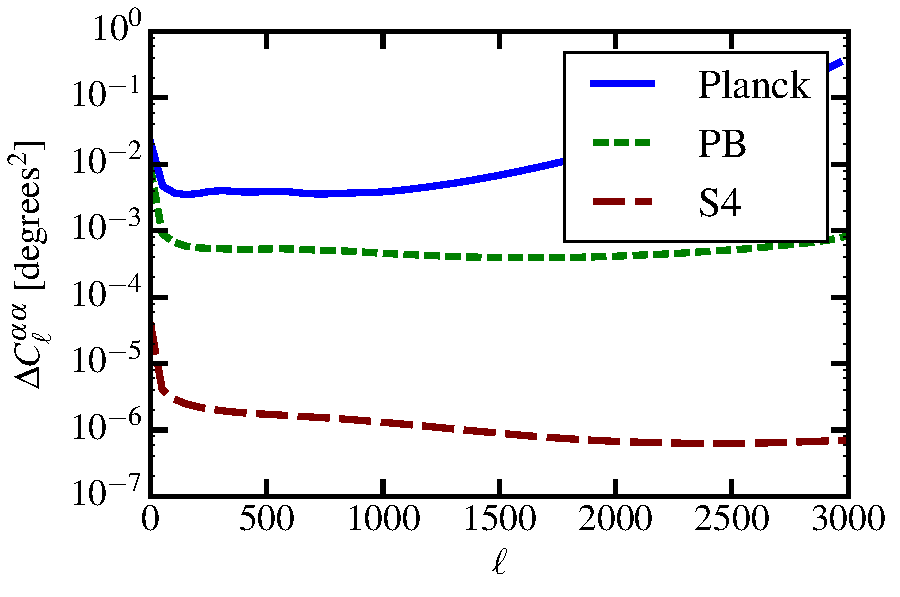
\includegraphics[width=0.70\textwidth]{BSMPhysics/birefringence-S4-planck-PB-v2.pdf}
\caption{The current (from POLARBEAR, labeled as PB) and projected (for Planck and Stage-IV experiment) 1$\sigma$ errobars on the birefringent rotation-angle power spectrum are shown on the vertical axis. A Stage-IV has the potential to improve the current best constraint on anisotropic birefringence by more than two orders of magnitude at all multipoles. For the Stage-IV forecast, we assumed noise of $1.41$ $\mu$K-arcmin (in polarization), a resolution of 1', and have considered polarization modes from $\ell=30$ to $\ell=5000$.}
\label{fig:CB-forecast}
\end{figure}

For a fixed integration time (and a varied noise level and sky coverage), large sky coverage optimizes sensitivity to low multipoles of the rotation angle and gives the best signal-to-noise ratio for rotation models that have power on large scales (such as, for example, a model with a scale-invariant power spectrum, which could result from fluctuations in a spectator scalar field present during inflation). Conversely, for models that have power on scales corresponding to multipoles above $\ell\sim 1000$, best signal-to-noise is achieved with deeper integration on small sky patches.  For a measurement of the magnitude of the quadrupole of the rotation angle, reducing the resolution from 1' to 9' produces a factor of a few increase in the projected errorbar (for all other parameters fixed). Increasing the noise from $1.41$ to $12.7$ $\mu$K-arcmin produces a factor of about $20$ increase in the errorbar. Access to polarization modes down to $\ell=2$ does not significantly affect the forecasts. 


\section{Primordial Magnetic Fields}

The origin of the microgauss ($\mu$G) strength magnetic fields in galaxies and galaxy clusters is one of the long standing puzzles in astrophysics \cite{Durrer:2013pga}. It is challenging to explain such fields based solely on the dynamo mechanism, without there being some initial seed field. However, if magnetic fields were present in the early universe, they would remain frozen in the cosmic plasma and collapse with the rest of the matter to form the galactic fields \cite{Grasso:2000wj}, or at least provide the seeds for the dynamo. A primordial magnetic field (PMF) could be produced in the aftermath of cosmic phase transitions \cite{Vachaspati:1991nm} or in specially designed inflationary scenarios \cite{Turner:1987bw,Ratra:1991bn}. Detecting their signatures in the CMB temperature and polarization would decisively prove their primordial origin. Aside from explaining the galactic fields, bounds on PMF have profound implications for our understanding of the early universe.  They help constrain theories of inflation \cite{Bonvin:2011dt}, models of the QCD and electroweak phase transitions \cite{Caprini:2007xq} and baryogenesis \cite{Vachaspati:2001nb}.

A stochastic PMF affects CMB in several ways. Magnetic stress-energy induces scalar, vector and tensor mode perturbations in the metric, and the Lorentz force generates vorticity in the photon-baryon fluid \cite{Subramanian:1998fn,Mack:2001gc,Lewis:2004ef,Shaw:2009nf,Paoletti:2010rx}. Dissipation of PMF on small scales dumps energy into the plasma, which produces spectral distortions and affects the recombination history \cite{Kunze:2014eka}.  Finally, Faraday Rotation (FR) of CMB polarization converts some of the $E$-modes into $B$-modes \cite{Kosowsky:2004zh,Pogosian:2011qv}.

Stochastic PMF has two potentially observable frequency independent contributions to the $B$-mode spectrum \cite{Shaw:2009nf}. One comes from the passive, or uncompensated tensor mode, which is generated by the PMF before neutrino decoupling. For nearly scale-invariant PMF, the spectrum of this component is indistinguishable from the inflationary gravity wave signal. The amplitude of this tensor contribution is proportional to $B^4_{1\rm{Mpc}} [\ln(a_\nu / a_{\rm{PMF}})]^2$, where $B_{1\rm{Mpc}}$ is the PMF strength smoothed over $1$Mpc, $a_\nu$ is the scale factor at neutrino decoupling and $a_{\rm{PMF}}$ is the scale factor at which PMF was generated. The other is the PMF vector mode which peaks at $l \sim 2000$, with the precise peak position dependent on the PMF spectrum. The vector-mode contribution is independent of $a_{\rm{PMF}}$. 

Planck data limits the magnetic field strength to $B_{1 {\rm Mpc}}<4.4$ nanogauss (nG) at the $95\%$ confidence level \cite{Ade:2015cva}. Similar bounds were recently obtained by POLARBEAR \cite{Ade:2015cao} based on their B-mode spectrum alone.

A Stage-IV experiment can improve the $95\%$ bound to 0.6 nG based on the PMF vector mode contribution to the B-mode spectrum. Comparable bounds can be obtained from the mode-coupling correlations induced by Faraday Rotation. The mode-coupling is the same as in the case of birefringence discussed in Sec.~\ref{sec-biref}, except for the Faraday Rotation being frequency dependent.

\section{Cosmic Strings}

\begin{table}[htbp!]\label{tab:string_forecast}
  \begin{center}
    \begin{tabular}{ c || c | c }
      \hline
       Model & Planck & CMB-S4 (1' resolution)  \\ \hline \hline
       Fixed $\alpha_\mathrm{str}:$ & $\sigma(f_{10})= 0.015$ & $\sigma(f_{10})=1.06\times 10^{-3}$  \\ \hline
       Varying $\alpha_\mathrm{str}:$ & $\sigma(f_{10})= 0.017$ & $\sigma(f_{10})=1.85\times 10^{-3}$ \\
        & $\sigma(\alpha_\mathrm{str})= 5.55$ & $\sigma(\alpha_\mathrm{str})=0.64$ \\\hline \hline
    \end{tabular}
  \end{center}
  \caption{Forecast constraints on the fraction of power in cosmic strings at $\ell=10$ and on the `wiggliness' of the string network, $\alpha$. {\it Planck} forecast is based on Blue Book values, with $f_{\rm sky} = 0.75$. CMB-S4 will yield an order of magnitude improvement in constraints on cosmic string parameters.}
\end{table}

Cosmic strings can at most contribute O(1\%) to the total CMB temperature anisotropy~\cite{Ade:2013xla,Lizarraga:2014xza,Lazanu:2014eya}, however, they can still generate observable B-modes. As shown in \cite{Moss:2014cra}, the bounds on cosmic strings obtained solely from the POLARBEAR \cite{Ade:2014afa} and BICEP2  \cite{Ade:2014xna} B-mode spectra are comparable to those from temperature spectra. 
We forecast the predicted constraints on cosmic strings using the StringFast code \cite{Foreman:2011uj}, based on the CMBACT simulations \cite{Pogosian:1999np} of a general string network, which allows for the correlation length of the strings, the `wiggliness' (which controls the small-scale structure of the string network) and the string rms velocity. StringFast allows for fast computation of the relevant string spectra, and includes the contribution to the string spectrum from scalar, vector and tensor modes, which are most relevant for the string B-modes \cite{Foreman:2011uj}.

In keeping with the methodology of recent results, we compute the string spectrum with a value of the string tension ($G_\mu/c^2=1.97\times10^{-6}$) that allows strings to make up all the TT power at $\ell=10$, and then use the fraction of the spectrum at that multipol $f_{10}$ as the forecast parameter. $f_10$ scales with the string tension as $f_{10} \propto G_\mu^2.$ The Fisher projections for Planck around a fiducial model of $f_{10}=0.01$ are $f_{10}<0.032,$ which maps to $G_\mu/c^2 < 3.5\times 10^{-7}\, 95\% \mathrm{CL}$, is consistent with the Planck constraints on the AH-mimic spectra.
We assume a fidcual model for the `wiggliness' $\alpha_\mathrm{str}$, string velocity $v_\mathrm{str}$ and correlation length $\xi_\mathrm{str}$ of $1.05, 0.4$ and $0.35$ respectively, in keeping with the model assumed in \cite{Foreman:2011uj}. We consider models where only the string fraction is varied, and the additional model where the small-scale structure of the string network is varied. The constraints are summarised in Table~\ref{tab:string_forecast} for a baseline resolution of 1 arcminute. The error on the string fraction for a 2 arcminute beam is only degraded by a few percent relative to the nominal case. In addition, the constraints are not strongly improved with the addition of BAO data, or with a more improved measurement of $\tau$.



